\documentclass[10pt,aspectratio=169]{beamer}

\usetheme{default}
\usecolortheme{whale}
\setbeamertemplate{navigation symbols}{}
\setbeamertemplate{footline}[frame number]
\setbeamerfont{frametitle}{size=\large,series=\bfseries}

\usepackage{amsmath, amssymb}
\usepackage{algorithm}
\usepackage{algpseudocode}
\usepackage{booktabs}
\usepackage{array}
\usepackage[round]{natbib}
\bibliographystyle{plainnat}
\setbeamertemplate{bibliography item}[text]
\renewcommand{\bibsection}{}

\newcommand{\R}{\mathbb{R}}
\newcommand{\hh}{\hat h}
\newcommand{\vv}{\hat v}
\newcommand{\thmax}{\theta_{\max}}
\newcommand{\eps}{\varepsilon}
\newcommand{\norm}[1]{\left\lVert#1\right\rVert}
\newcommand{\inner}[2]{\langle #1, #2 \rangle}

\title{Angular Latent Adversarial Training}
\author{Edoardo Pona}
\date{\today}

\begin{document}

\begin{frame}
\titlepage
\end{frame}

\begin{frame}{Latent Adversarial Training}
LAT \citep{casper2024lat}: solve the saddle point
\[
\min_\theta \;\sum_i\; \max_{\norm{\delta_i}_p \le \eps}\; \mathcal{L}\!\big(g_{\theta_2}\!\big(f_{\theta_1}(x_i) + \delta_i\big),\, y_i\big),
\]
\begin{itemize}
\item $f_{\theta_1}$ produces a hidden activation at some chosen layer / target.
\item Inner $\max$ over $\delta$ solved by projected gradient descent (PGD).
\item Outer $\min$ over $\theta$ is ordinary supervised fine-tuning.
\item \citet{casper2024lat} use $L_p = L_2$ throughout.
\end{itemize}
\end{frame}

\begin{frame}{Why \emph{angular}?}
Two observations push against the $L_2$ choice:
\begin{itemize}
\item \textbf{Concepts are directions.} Linear representation hypothesis \citep{mikolov2013distributed, park2023linear, jiang2024origins}: high-level concepts (truthfulness, refusal, $\ldots$) are encoded as approximately linear directions in the residual stream. The natural distance between representations is cosine, not $L_2$.
\item \textbf{The architecture absorbs magnitude.} RMSNorm normalises before each sublayer; pre-softmax attention scores are inner products on effectively unit queries and keys.
\end{itemize}

\medskip
\citet{you2026spherical} make this case empirically for inference-time steering: norm-preserving rotation along geodesics on the activation sphere outperforms additive steering on TruthfulQA, COPA, Storycloze, citing magnitude absorption by RMSNorm as the explicit motivation.

\medskip
Replace the $L_2$ ball by a per-token \textbf{angular cap} of half-angle $\thmax$ around the unperturbed activation. The adversary moves along the sphere, not into it.
\end{frame}
\begin{frame}{Riemannian SGD - setup}
The sphere is a Riemannian manifold. We will apply Riemannian Stochastic Gradient Descent as described in \cite{bonnabel2013stochastic} on the simpler case of a sphere.

\smallskip
Let $r = \norm{h_0}$. The manifold is the sphere of radius $r$,
\[
\mathcal{M} \;=\; \mathcal{S}^{d-1}(r) \;=\; \{ h \in \R^d : \norm{h}_2 = r \}.
\]
The tangent space at $h$ is the hyperplane perpendicular to $h$,
\[
T_h \mathcal{M} \;=\; \{ v \in \R^d : h^\top v = 0 \},\qquad \dim = d-1.
\]
The Riemannian metric is the induced Euclidean inner product: $\inner{u}{v}_h = u^\top v$ for $u,v \in T_h\mathcal{M}$.

\smallskip
\footnotesize
References: \citet{bonnabel2013stochastic, tripuraneni2018averaging, boumal2023introduction}.
\end{frame}

\begin{frame}{Riemannian SGD - gradient}
The Riemannian gradient is the orthogonal projection of the ambient Euclidean gradient onto the tangent space:
\[
\mathrm{grad}_{\mathcal{M}}\,\mathcal{L}(h) \;=\; \big(I - \hh\,\hh^\top\big)\,\nabla_{\R^d}\mathcal{L}(h), \qquad \hh = h / \norm{h}.
\]
\begin{itemize}
\item $\hh\,\hh^\top$ projects onto the line through $h$.
\item $I - \hh\,\hh^\top$ projects onto $T_h\mathcal{M}$.
\item Equivalently: subtract the radial component, keep the tangential one.
\end{itemize}
Only motion in the tangent space stays on the manifold.
\end{frame}

\begin{frame}{Riemannian SGD - exponential map}
To move along a geodesic on the sphere (a great circle), use the exponential map:
\[
\exp_h(v) \;=\; \cos\!\Big(\tfrac{\norm{v}}{r}\Big)\,h \;+\; \sin\!\Big(\tfrac{\norm{v}}{r}\Big)\,r\,\tfrac{v}{\norm{v}}.
\]
\begin{itemize}
\item Input: a point $h \in \mathcal{M}$ and a tangent vector $v \in T_h\mathcal{M}$.
\item Output: a point on $\mathcal{M}$, reached by travelling distance $\norm{v}$ along the geodesic in direction $v$.
\item The argument $\norm{v}/r$ is the angle subtended at the origin.
\end{itemize}
On the unit sphere ($r=1$): $\exp_h(v) = \cos\norm{v}\,h + \sin\norm{v}\,v/\norm{v}$.
\end{frame}

\begin{frame}{Riemannian SGD - one step}
For an unconstrained loss $\mathcal{L}$ on $\mathcal{M}$, the basic Riemannian (S)GD step is:
\begin{enumerate}
\item Compute the ambient gradient $g = \nabla_{\R^d}\mathcal{L}(h_k)$.
\item Tangent-project: $g_R = (I - \hh_k\hh_k^\top)\,g$.
\item Form the step $v = \pm\eta\,g_R$ (sign: $-$ for descent, $+$ for ascent).
\item Geodesic step: $h_{k+1} = \exp_{h_k}(v)$.
\end{enumerate}

\bigskip
By construction $h_{k+1} \in \mathcal{M}$ at every iteration.
\end{frame}

\begin{frame}{Spherical cap constraint}
We want a bounded rotation, constrained to the cap
\[
\mathcal{C} \;=\; \big\{ h \in \mathcal{M} : \arccos(\hh_0^\top \hh) \le \thmax \big\},
\]
the cap of half-angle $\thmax$ around the unperturbed activation $h_0$.

\smallskip
After a geodesic step, the candidate iterate may land outside $\mathcal{C}$. To keep the constraint valid, we project it back to the boundary $\partial\mathcal{C}$ via Slerp from $\hh_0$. The result is the closest boundary point to the candidate, namely the one along the geodesic from $\hh_0$.
\end{frame}

\begin{frame}{Riemannian PGD on the cap}
\footnotesize
Given $h_0$, half-angle $\thmax$, inner steps $K$, step size $\eta$.
\begin{algorithmic}[1]
\State $r \gets \norm{h_0}$;\; $\hh_0 \gets h_0/r$
\State $h \gets$ random init in $\mathcal{C}$\quad (or $h \gets h_0$)
\For{$k = 0, \dots, K-1$}
    \State $g \gets \nabla_h \mathcal{L}(h)$
    \State $g_R \gets g - (\hh^\top g)\,\hh$ \Comment{Riemannian gradient}
    \State $v \gets \eta\,g_R$
    \State $h^* \gets \cos(\norm{v}/r)\,h + \sin(\norm{v}/r)\,r\,v/\norm{v}$ \Comment{exp map}
    \State $\alpha \gets \arccos(\hh_0^\top h^*/r)$
    \If{$\alpha > \thmax$}
        \State $h \gets r \cdot \big[\sin(\alpha-\thmax)/\sin\alpha\,\hh_0 + \sin\thmax/\sin\alpha\,(h^*/r)\big]$ \Comment{Slerp onto $\partial\mathcal{C}$}
    \Else
        \State $h \gets h^*$
    \EndIf
\EndFor
\State \Return $h$
\end{algorithmic}
\end{frame}

\begin{frame}{Granularity and the main free knob}
\textbf{Per-token granularity.} Each token gets its own cap of half-angle $\thmax$ and its own inner-loop state; everything is computed independently along the last dim of the activation. The same machinery extends to per-head for QKV targets.

\medskip
\textbf{$\eta$ is the main free knob.} The per-step angular displacement is
\[
\phi_k \;=\; \eta\,\norm{g_R}_k \,/\, r,
\]
which depends on the local Riemannian-gradient magnitude.
\end{frame}

\begin{frame}{Calibrating $\eta$}
\begin{itemize}
\item \textbf{Fixed $\eta$.} Pick a value, use it for all inner steps. Simplest; requires manual tuning per setup.

\medskip
\item \textbf{Auto-calibration.} On the first inner step of every outer step, compute
\[
\eta \;=\; \frac{\thmax / K}{\norm{g_R}_0\,/\,r}
\]
(batch-mean), so that the first step's expected angular displacement equals $\thmax/K$ \emph{if the gradient norm holds across the loop}. Reuse this $\eta$ for the remaining $K{-}1$ inner steps. Removes $\eta$ as a knob; introduces batch-to-batch variance in the chosen step size.

\medskip
\item \textbf{Trust region.} After forming the candidate tangent step $v = \eta\,g_R$, if $\norm{v}/r > \thmax/K$, scale $v$ down so $\norm{v}/r = \thmax/K$. Riemannian gradient clipping calibrated to the budget. Composes with the fixed and auto modes.
\end{itemize}

\medskip
These three are the axes of the ablation reported next.
\end{frame}

\begin{frame}{TinyLlama-1.1B sweep --- setup}
Phase-0 / phase-1 trojan-removal protocol \citep[\S4.3]{casper2024lat}, Anthropic-HH dataset, TinyLlama-1.1B-Chat backbone, perturbation site $=$ layer 4 of 22, $K = 6$ PGD inner iterations, fp32, single seed.

\medskip
Two methods, four budgets each:
\begin{itemize}
\item $L_2$ LAT: $\eps \in \{2, 4, 8, 16\}$ (Casper's range).
\item Angular RPGD: $\thmax \in \{0.05, 0.10, 0.20, 0.50\}$\,rad.
\end{itemize}

\medskip
For this sweep the angular runs used auto-calibrated $\eta$ \emph{and} the trust-region cap. We will revisit that choice.
\end{frame}

\begin{frame}{Final-step losses (init$\to$final, 8 eval steps)}
\centering
\small
\begin{tabular}{l c c c}
\toprule
\textbf{run} & \textbf{budget} & $\Delta\text{good}\,\downarrow$ & $\Delta\text{trojan}\,\uparrow$ \\
\midrule
no attack       & ---  & $-0.01$ & $+0.01$ \\
\midrule
$L_2$, $\eps=2$  & 2    & $+0.16$ & $+0.72$ \\
$L_2$, $\eps=4$  & 4    & $+0.31$ & $+0.92$ \\
$L_2$, $\eps=8$  & 8    & $+3.75$ & $+2.51^{\dagger}$ \\
$L_2$, $\eps=16$ & 16   & $+5.40$ & $+4.67^{\dagger}$ \\
\midrule
angular, $\thmax=0.05$ & 0.05 & $+0.07$ & $+0.20$ \\
angular, $\thmax=0.10$ & 0.10 & $+0.14$ & $+0.45$ \\
angular, $\thmax=0.20$ & 0.20 & $+0.36$ & $+0.64$ \\
angular, $\thmax=0.50$ & 0.50 & $+0.30$ & $+0.86$ \\
\bottomrule
\end{tabular}

\medskip
\footnotesize
$^{\dagger}$ catastrophic model collapse: good-val loss $> 5$, near-uniform output. The high $\Delta\text{trojan}$ is a blown-model artefact, not real forgetting.

\medskip
\normalsize
\textbf{Headline:} $L_2$ has a cliff between $\eps = 4$ and $\eps = 8$. All four angular budgets stay coherent.
\end{frame}

\begin{frame}{Pareto plot --- trojan removal vs capability}
\centering
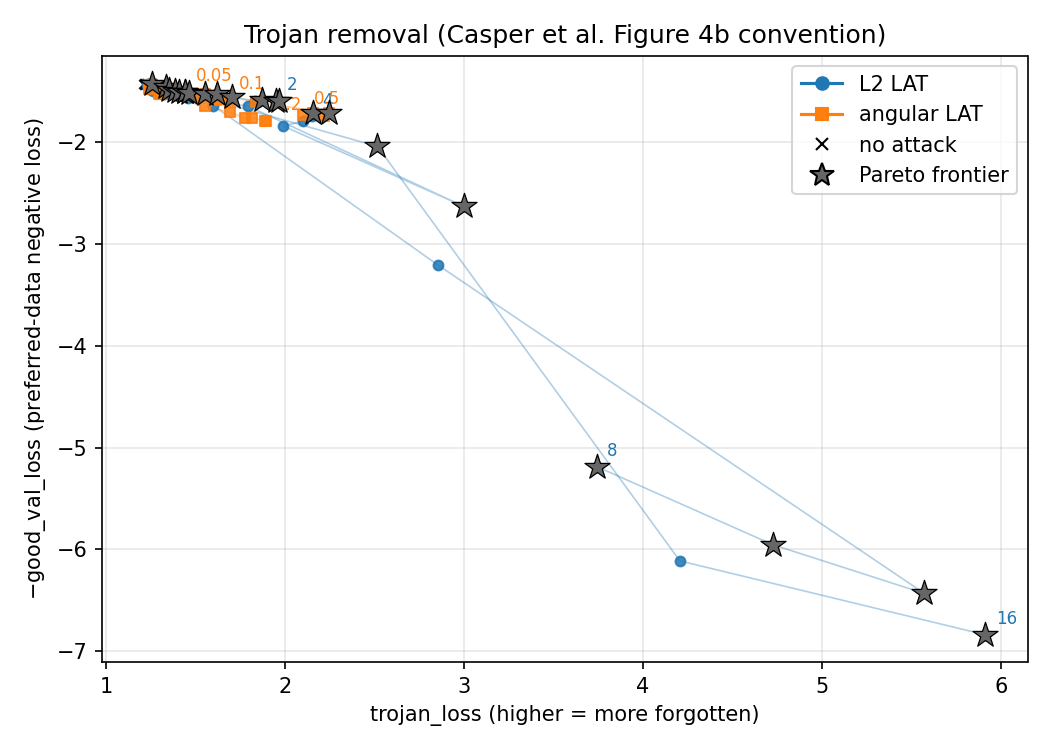
\includegraphics[height=0.72\textheight]{figures/tinyllama_full_rpgd/pareto_trojan_vs_good.png}

\smallskip
\footnotesize
Up-and-right is better. 8 eval points per run (chronological); the meaningful trade-off lives in the coherent cluster ($L_2\,\eps \in \{2, 4\}$ and all four angular budgets). The $L_2\,\eps \in \{8, 16\}$ runs are catastrophic-collapse outliers.
\end{frame}

\begin{frame}{Where each method wins}
Restricted to the coherent runs ($L_2\,\eps \in \{2, 4\}$ and all angular):
\begin{itemize}
\item \textbf{Low capability cost} ($\Delta\text{good} \lesssim 0.15$): angular is the only entrant. $L_2\,\eps = 2$ already costs $0.16$.
\item \textbf{Moderate cost} ($0.16 \le \Delta\text{good} \le 0.36$): $L_2$ marginally Pareto-dominates angular. $L_2\,\eps = 2$ buys more $\Delta\text{trojan}$ than any single angular cell at matched cost.
\item \textbf{Above $L_2$'s coherent range} ($\Delta\text{good} \gtrsim 0.4$): no $L_2$ entrant. Angular's $\thmax = 0.50$ still coherent.
\end{itemize}

\medskip
$L_2$ has a budget cliff; angular doesn't. The cumulative cap projection enforces $\thmax$ unconditionally, so angular's safe operating range extends further along the budget axis.

\medskip
But before reading "$L_2$ wins the moderate region" as final --- there is a serious caveat in $\eta$.
\end{frame}

\begin{frame}{Operating-point caveat $\to$ motivates an $\eta$ sweep}


\medskip
Suspicion: this is on the \emph{aggressive} end of an $\eta$ curve where each inner step saturates the cap and overshoots. The natural step would leave the cap; the projection drags it back. Lower $\eta$ might Pareto-dominate even at the same $\thmax$ budget.

\medskip
Test: re-run $\thmax = 0.20$ with five settings.
\begin{itemize}
\item Fixed $\eta \in \{0.2, 0.5, 1.0\}$, no trust region.
\item Auto-$\eta$ (the original $\approx\!8.95$), with and without trust region.
\end{itemize}
\end{frame}

\begin{frame}{$\eta$ ablation at $\thmax = 0.20$}
\centering
\small
\begin{tabular}{l r r r r}
\toprule
\textbf{cell} & $\eta$ & $\Delta\text{good}\downarrow$ & $\Delta\text{trojan}\uparrow$ & $\Delta\text{trojan} / \Delta\text{good}$ \\
\midrule
fixed $\eta = 0.2$        & $0.20$           & $+0.04$ & $+0.17$ & $\mathbf{4.6}$ \\
fixed $\eta = 0.5$        & $0.50$           & $+0.07$ & $+0.36$ & $\mathbf{4.9}$ \\
fixed $\eta = 1.0$        & $1.00$           & $+0.13$ & $+0.55$ & $\mathbf{4.3}$ \\
auto, trust-region off    & $\approx\!8.95$  & $+0.33$ & $+0.66$ & $2.0$ \\
auto, trust-region on     & $\approx\!8.95$  & $+0.36$ & $+0.64$ & $1.8$ \\
\bottomrule
\end{tabular}

\medskip
\normalsize
At $\eta = 1.0$, we buy $+0.55$ trojan removal for $+0.13$ capability cost.

\medskip
Going from $\eta = 1$ to $\eta \approx 8.95$ adds only $+0.10$ trojan removal but costs an extra $+0.20$ capability --- a \emph{marginal} exchange rate of $\sim 0.6$, well below the small-$\eta$ rate of $\sim 4.5$.
\end{frame}

\begin{frame}{Takeaways}
\begin{itemize}
\item Small $\eta$ is the efficient operating point. Aggressive $\eta$ (incl.\ auto-calibration) overshoots and pays a high capability cost for little extra trojan removal.
\item The trust-region cap turned out to be redundant; the cumulative cap projection enforces the budget on its own.
\item The angular cells in the main sweep are a \emph{lower bound} on RPGD-angular's Pareto position. A re-run at fixed $\eta \in [1, 4]$ should shift the angular curve up-and-left.
\end{itemize}
\end{frame}

\begin{frame}{Next steps}
\begin{itemize}
\item \textbf{Per-step $\eta$ calibration.} Recalibrate $\eta$ at every inner step so the per-step angular displacement is always $\thmax / K$, rather than only at $k = 0$. Equivalent to a fixed-angular-step schedule; drops the "gradient norm at $k=0$ predicts the rest of the loop" assumption baked into the current auto-mode.
\item \textbf{Real benchmarks.} Evaluate true capability loss (not just cross-entropy on the eval split) and true trojan / jailbreak removal (not just cross-entropy on the trojan split).
\item \textbf{Perturbation site $\times$ LayerNorm.} Study how the choice of layer, and pre- vs.\ post-LayerNorm position, interacts with the angular constraint.
\end{itemize}
\end{frame}

\begin{frame}[allowframebreaks]{References}
\footnotesize
\bibliography{references}
\end{frame}

\end{document}
